\section{Entreprise et environnement de travail}

\subsection{Présentation de l'entreprise}

Le groupe Excilys regroupe sept SSII, toutes concentrées autour des technologies Java/JEE : 
\begin{itemize}
	\item eBusiness Information
	\item Altendis
	\item SS2J
	\item Equitalis
	\item Adlys
	\item Visual3X
	\item eAdvance
\end{itemize}

\subsubsection{L'excellence technique}
Le groupe Excilys a fait le choix de propser à ces clients (parmi lesquels on peut des sociétés du CAC 40) des consultants à la tarification certes plus élévée, mais dont la compétence et le savoir technique sont supérieurs à la concurrence.\\

Cette orientation se retrouve dans le mode de recrutement du groupe Excilys : la plupart des consultants sont recrutés dans le cadre de leur stage de fin d'études.\\
Le groupe Excilys utilise en effet cette période pour compléter leur formation à la fois théorique et pratique et souvent leur donner en plus une première expérience de projet client.\\

Le groupe a également fortement investi dans un système de capitalisation des
connaissances développé en interne - Capico - , pour que chaque consultant puisse partager ses connaissances techniques, consulter les fiches existantes ou encore évaluer ses compétences. Etant donné la stratégie du groupe résolument tournée vers l’excellence, ce système de partage des connaissances est fondamental et focalise un budget conséquent de recherche et développement.\\

Le groupe Excilys intervient auprès de ses clients aussi bien pour du développement que de l'audit ou de la formation.\\

\subsubsection{Le Service Equitable}

Au-delà de tous les outils qui sont mis à disposition des consultants du groupe, c’est avant tout la Charte qui constitue sa véritable identité et fédère à la fois ses consultants et ses clients. Le modèle des plus singuliers sur la place est pourtant des plus pragmatiques. Des règles de bonne conduite, la volonté que chaque acteur soit respecté dans ses attentes et respecte lui aussi les autres et une meilleure répartition des rémunérations entre tous, notamment pour le consultant.

\begin{figure}[h!]
	\centering
		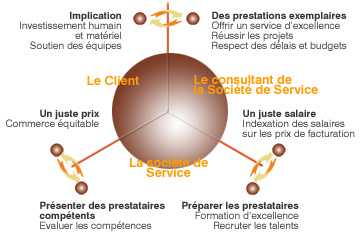
\includegraphics[scale=1]{service-equitable.jpg}
	\caption{Le Service Equitable}
\end{figure}

Pour créer cette rétroaction entre le client et les consultants, le groupe a ainsi adopté la règle dite des 60/40, qui permet de reverser aux consultants hors frais commerciaux sous forme de primes 60\% des facturations. Les consultants du groupe bénéficient ainsi de rémunérations élevées, mais en accord avec ce que l’implication et la qualité de leur travail apporte.

\subsection{Environnement de travail}

L'environnement de travail est celui d'une SSII \og classique \fg{} : l'open space, afin de faciliter la communication entre développeurs, au coeur de la méthode Scrum qui est la méthode de travail privilégiée par le Groupe.\\
Comme indiqué précedemment, le mode de recrutement  d'Excilys se basant principalement sur le recrutement de stagiaires en fin d'études, une vingtaine de stagaires ont été pris cette année. Cela m'a conduit avec travailler surtout avec des personnes dans la même situation que moi, ce qui a grandement facilité la communication et le partage de connaissances, car nous avions tous à y gagner : la société se prépare à éventuellement engager l'ensemble des stagaires, il n'y a donc pas eu de phénomène de compétition entre stagiaires, ce qui aurait pu conduire à un cadre de travail délétère.\\

Le groupe Excilys restant malgré tout une SSII de petite taille (environ une centaine de personnes), je n'y ai pas trouvé le type de hiérarchie pyramidale commun aux grandes SSII. Au contraire l'ensemble des directeurs a été très disponible et à l'écoute.\\

Globalement, le cadre de travail fut des plus agréables et ce fut pour moi un réel plaisir de travailler pendant ces 6 derniers mois avec l'ensemble du personnel.

\subsubsection{Intégration au sein de l'entreprise}

Les informations fournies au début du stage m’ont permis de comprendre et de gérer rapidement les aspects administratifs du stage (horaires, feuilles de temps, congés. . .) ainsi que de démarrer rapidement la formation de 2 mois.\\
Cette longue phase de formation a conduit à une intégration tardive dans une équipe, puisque celle-ci n’est intervenue qu'à la fin du premier mois, lors du démarrage du projet en interne (6 personnes). Les objectifs de travail ont été clairement  énoncés dès le départ :
\begin{itemize}
	\item Suivre la formation Capico lors du premier mois.
	\item Réaliser les fonctionnalités demandées durant le projet en interne le second mois.
	\item Une fois l'équipe Gatling intégrée, Réaliser les nouvelles fonctionnalités demandées.
	\item Passer la certification OCPJP durant le stage (obtenue avec 91\% de bonnes réponses)
\end{itemize} 
Le support a été essentiellement Capico, qui a servi à la fois de livret d’accueil et de plateforme de formation.\\

L'intégration au sein de l'entreprise a été grandement simplifiée par les employés d'Excilys, toujours disponibles lorsque j'ai pu rencontrer un problème technique.\\